\documentclass[12pt]{report}   % SUBMISSION TO GRAD SCHOOL
%\documentclass[12pt,twoside]{report}  % TWOSIDE DUPLEX OUTPUT
\usepackage{setspace}
\usepackage{buthesis}
\usepackage{amsmath,amssymb,graphicx,amsfonts,amsthm}
\usepackage{verbatim}
\usepackage{epsfig}
\usepackage{wrapfig}
\usepackage{latexsym,amsfonts,amscd}
\usepackage{changebar}
\usepackage{enumerate}
% Do you use TikZ?
\usepackage{tikz}
%\usepackage{pgfmath}
\usetikzlibrary{decorations}
\usetikzlibrary{shadows}

% Used only for example text
\usepackage{lipsum}

\usepackage[footnotesize,bf]{caption}  % Reduces caption font sizes

%%%%%%%%%%%%%%%%% Fancy chapter headings %%%%%%%%%%%%%%%%%%%
\usepackage[Bjarne]{ThesisFncychap}
% Redefine alphano commands

%%%%%%%%%%%%%%%%%%%%%%%%%%%%%%%%%%%%%%%%%%%%%%%%%%%
\makeatletter
  
  \ChNameVar{\Huge\sc}    % sets the style for name
  \ChNumVar{\Huge\sc}         % sets the style for digit
  \ChTitleVar{\Huge\bf\centering} % sets the style for title
  \ChRuleWidth{4pt}        % Set RW=4pt
  %\ChNameUpperCase         % Make name uppercase
  \ChNameAsIs         % Make name uppercase
  \ChTitleAsIs

  \renewcommand{\DOCH}{%
    %\setlength{\fboxrule}{\RW} % Let fbox lines be controlled by
                               % \ChRuleWidth
    %\fbox{\CNV\FmN{\@chapapp}\space \CNoV\thechapter}\par\nobreak
    \thispagestyle{empty}
    \vskip 80\p@
    \begin{center}
    %\CNV\FmN{\@chapapp}\space \CNoV\thechapter\par\nobreak
    \CNV\FmN{\@chapapp} \TheAlphaChapter\par\nobreak
    \begin{tabular*}{\textwidth}{c}
      \hline
    \end{tabular*}
    %\line(1,0){5in}\\
    \end{center}
    %\vskip 20\p@
    }

  \renewcommand{\DOTI}[1]{%
    \CTV\FmTi{#1}\par\nobreak
    \vskip 40\p@
    {\newpage}
    }
  \renewcommand{\DOTIS}[1]{%
    \CTV\FmTi{#1}\par\nobreak
    \vskip 40\p@
    }
\makeatother


%%%%%%%%%%%%%%%%%%%%%%%%%%%%%%%%%%%%%%%%%%%%%%%%%%%%%%%%%%%%

%-----------------------------------------------------------------
%% Control the fonts and formatting used in the table of contents, list of
%% figures, and list of tables
\usepackage[titles]{tocloft}
%\newcommand{\del}{\partial}
\graphicspath{ {images/}}


\newcommand{\by}{\mathbf{y}}
\newcommand{\bx}{{\boldsymbol{\hat{x}}}}
\newcommand{\bn}{{\boldsymbol{\hat{n}}}}
\newcommand{\bt}{{\boldsymbol{\hat{t}}}}
\newcommand{\bu}{\mathbf{u}}
\newcommand{\grad}{\mathbf{\nabla}}
\newcommand{\del}{\partial}
\newcommand{\hg}{h_g}
\newcommand{\Rey}{{R}}
\newcommand{\Ndg}{\tilde{N}_g}
\newcommand{\monami}{\textit{monami}}
\newcommand{\ubl}{U_\text{bl}}
\newcommand{\words}[1]{\textbf{(#1)~}}
% \newcommand{\words}[1]{{}}
\newcommand{\ReyNdg}{{\Rey\Ndg}}






\renewcommand{\bar}{\overline}

%% Aesthetic spacing redefines that look nicer to me than the defaults.
\setlength{\cftbeforechapskip}{-1ex}
\setlength{\cftbeforesecskip}{-3.5ex}
\setlength{\cftbeforesubsecskip}{-3.5ex}
\setlength{\cftbeforetabskip}{-3.5ex}
\setlength{\cftbeforefigskip}{-3.5ex}
%-----------------------------------------------------------------

\dissertation % This *is* what you're writing, right?

% Information about the document
%-----------------------------------------------------------------
\title{
Hydrodynamic instability leading to \textit{Monami}
}
\author{Ravi Shanker Singh}
\degree{Doctor of Philosophy}
\department{Department of Physics}
\previousdegrees{
		B.Sc., Banaras Hindu University; Varansi, India, 2006\\ 
		M.Sc.(Physics), Indian Institute of Technology-Bombay; Mumbai, India, 2008}	
\thesismonth{May} \thesisyear{2014}
%-----------------------------------------------------------------

\begin{document}

\doublespacing
\begin{preliminaries}
\maketitle

\copyrightpage

\begin{signature}
  \director{Shreyas Mandre, Ph.D., Advisor}
  \reader{J. Tang, Ph.D., Reader}
  \reader{Tom Powers, Ph.D., Reader}
\end{signature}

\begin{vita}
  %\lipsum[1-2]

  %xzczxl;csd ;vdfsvl;sd
\end{vita}

\begin{acknowledgments}
 % \lipsum[3-4]

\end{acknowledgments}

\begin{abstract}
 % \lipsum[6-8]

  \thispagestyle{empty}
  % Do you want this page to exist in the numbering?
%  \thispagestyle{empty}
%  \if@twoside
%    \addtocounter{page}{-2}  
%  \else
%    \addtocounter{page}{-1}
%  \fi
\end{abstract}

% Why double-space toc,lof, and lot?
\begin{spacing}{1}
  \tableofcontents
  \clearpage{\pagestyle{empty}\cleardoublepage}

  \footnotesize
  \fontsize{11.5pt}{12.5pt}\selectfont
  \listoftables
  \clearpage{\pagestyle{empty}\cleardoublepage}

  \listoffigures
  \clearpage{\pagestyle{empty}\cleardoublepage}
  \normalsize
\end{spacing}

\end{preliminaries}

\pagestyle{myheadings}

%------------------------ CONTENT ------------------------%

\chapter{Introduction}
Seagrasses are submerged flowering plants found in shallow marine waters, mostly in the littoral zones of freshwater and in large expanses of low lying coastal shore, they occupy less than $0.05\%$ of the ocean areas but contribute directly to about $15\%$ of the total biomass production in the ocean. Seagrasses plays crucial role in protecting sea shores. The extensive root system in seagrasses, which extends both vertically and horizontally, helps stabilize the sea bottom in a manner similar to the way land grasses prevent soil erosion. With no seagrasses to diminish the force of the currents along the bottom, numerous beaches, businesses, and homes can be subject to greater damage from storms.
%ocean bottom areas which are mostly devoid of seagrass are vulnerable to intense wave action from currents and storms. 

Seagrasses provide food, shelter, and essential nursery areas to commercial and recreational fishery species and to countless invertebrates living in seagrass communities.
Some fish, such as seahorses and lizardfish, can be found in seagrasses throughout the year, while other fish remain in seagrass beds during certain life stages. While some organisms, including the endangered Florida manatee and green sea turtle, graze directly on seagrass leaves, others use seagrasses indirectly to provide nutrients. Bottlenose dolphins are often found feeding on organisms that live in seagrass areas. Detritus from bacterial decomposition of dead seagrass plants provides food for worms, sea cucumbers, crabs, and filter feeders such as anemones and ascidians. Further decomposition releases nutrients (such as nitrogen and phosphorus), which, when dissolved in water, are re-absorbed by seagrasses and phytoplankton.

The relative safety of seagrass meadows provides an ideal environment for the female fishes to to lay and hatch their eggs. The safety of seagrass meadows are also useful for the juvenile fish and invertebrates to conceal themselves from predators. Seagrass leaves are also ideal for the attachment of larvae and eggs, including those of the sea squirt and mollusk. Much of Florida's recreationally and commercially important marine life can be found in seagrass meadows during at least one early life stage. While seagrasses are ideal for juvenile and small adult fish for escape from larger predators, many infaunal organisms (animals living in soft sea bottom sediments) also live within seagrass meadows. Species such as clams, worms, crabs, and echinoderms, like starfishes, sea cucumbers, and sea urchins, use the buffering capabilities of seagrasses to provide a refuge from strong currents. The dense network of roots established by seagrasses also helps deter predators from digging through the substratum to find 
infaunal prey organisms. Seagrass leaves provide a place of anchor for seaweeds and for filter-feeding animals like bryozoans, sponges, and forams.

Seagrasses help trap fine sediments and particles that are suspended in the water column, which increases water clarity. When a sea floor area lacks seagrass communities, the sediments are more frequently stirred by wind and waves, decreasing water clarity, affecting marine animal behavior, and generally decreasing the recreational quality of coastal areas. Seagrasses are also known to sequester $C O_2$, mix and recycle the nutrients necessary for life of its inhabitants they also work to filter nutrients that come from land-based industrial discharge and stormwater runoff before these nutrients are washed out to sea and to other sensitive habitats such as coral reefs.
%However these ecosystems are disappearing at an alarming rate (average $7\%$ since 1990).

The primary requirement for active marine eco-systems are presence of sunlight and a mechanism to mix and transport the nutrients. Since sunlight can penetrate only near the surface of water, the sea-shores are ideal place for rich marine ecology. One of the other important factor in proliferating the marine ecology near the ocean shores is the presence of regular wave and tides which constantly stir the region, a mechanism which is not present in the lakes. Despite shallow average depth of lakes (e.g. average depth of Lake Erie is 18.6m and that of lake Chand is 4 m) with plenty of sunlight, lakes are not able to support a rich ecology as compared to the coastal shore due to absence of tidal mixing. The coastal oceans are about 10 times as productive as the lakes. Along with marshes and mangroves, seagrasses meadows rank highest in terms of biomass production.
\newline
%\newline
The ability of seagrass meadows to engineer the habitat for effective ecosystems is directly related to its ability to influence hydrodynamic processes. This requires balance between
two competing requirements such as flow should be sufficiently slow so that species don't get flushed along with the water, but not stagnant and thus allowing the nutrients and other material to be transported by the flow. It is widely believed that many systems including seagrass rely on flow for the transportation and mixing of nutrients, pollens, sperms etc. A simple estimate of mixing-strength in absence of any flow instability can be estimated to help us understand the importance of existence of flow instability. A typical seagrass patch extend from $10^2 m$ to $10^3 m$ with a typical flow speed of $0.1 m/s$ to $1 m/s$, indicating that any tracer particle carried by the flow would take about $\tau = 10^2-10^4 s$ to cross the patch. In the absence of any flow instability mean flow is horizontal and vertical transportation and mixing of material can happen only through turbulent diffusivity $\kappa =  0.1 U d$, where $ U \approx 1 cm/s$ is the mean flow in canopy, and $d \approx 1cm $ is characteristic 
length scale of plant such as its diameter or leave with. This estimate indicates that transportation of material above the grass bed can only penetrate about $\sqrt{\kappa \tau} = 3-30 mm $, compared to the canopy height of 10-100 cm. However in presence of flow instability even a modest $10\%$ conversion of horizontal flow to vertical velocity results in penetration length scale of about 10-1000 cm. Indeed, It is widely believed that the phenomenon of large amplitude coherent oscillation of marine grass, known as \textit{Monami} is a result of flow instability, much like coherent waves commonly observed on terrestrial grass field, known as \textit{Honami} in strong wind. While the two cases seems superficially similar, there are major difference such as atmospheric flow is essentially unbounded. Another major difference the two is the considerable difference of stiffness of canopies.
\newline
%from   assuming the plant diameter to be  exhibit rich set of dynamical behavior due to their interaction with the flow of water. The hydrodynamic processes resulting from these behavior are known to influence
%number of environmental processes such as transportation and mixing of sediments, contaminants, dissolved oxygen etc. One such response of submerged grass
%vegetation in response to unidirectional steady current is the large amplitude coherent oscillations, known as \textit{Monami}, which have been observed in laboratory(Ikedea, Nepf) as well as in observation of seagrass meadows in field studies (Kensworthy, Grizzle). Transportation and mixing of nutrients in dense canopies are known to be dominated by the phenomenon of \textit{Monami} which directly influences biomass production of marine plants as well as inhabitants of grass bed. 
%Similar phenomenon of large amplitude coherent oscillations are also observed for terrestrial canopies which are known as \textit{Honami}. A crucial difference between the atmospheric and aquatic flow is that the atmospheric are essentially unbounded vertically.
While considerable research is done to understand the phenomenon associated terrestrial canopies, research for the case of vegetation in water is not prevalent. The most notable of research work related to \textit{Monami} are laboratories study of open channel flow through flexible and rigid canopies(Nepf, Ikeda ), which shows existence of coherent eddies(refer to figure) propagating on canopy top. A systematic study on the topic of blue mussels larvae settlement attributed the excess presence of blue-muscel larvae on the tip of grass to the presence of \textit{Monami} (Grizzle 1996). Evidence of the effect of aquatic plants on unidirectional flow also emerges from the study of research groups interested in conveyance of water through vegetated canals (Kouwen 1992), the cycling of particulate and dissolved matter etc. 
\newline The current explanation of \textit{Monami} is inspired by the work of Raupach for the case of terrestrial canopies. Existing explanation invokes the existence of strong shear near the canopy top due to different amount of drag experienced by the flow with in and above the canopy. This shear layer is assumed to become unstable to coherent vertices through a mechanism similar to 
Kelvin-Helmholtz instability. Influence of these coherent eddies over sea grasses is manifested in their large amplitude synchronous oscillations.
While shear model successfully predicts the frequency of mo-nami for number of experimental observations (Nepf paper), several aspects of existing theory remain unexplained. First, the assumption of instability of perturbation to shear layer through a mechanism of Kelvin-Helmholtz relies on absence of any interaction between the flow perturbation and drag, making shear layer a inconsistent theory. Second, classical free shear flow is known to be unstable for all the Reynolds number. On the contrary estimated critical Reynolds number for lab scale and field observation are much higher $\approx O(1000)$. These drawbacks of existing theory suggest that flow through vegetation requires further investigation for better understanding of phenomenon.
\newline
In this study, we developed a mathematical model for the linear stability incorporating presence of grass through a drag field in the momentum equation of fluid. Although monami is mainfested in the motion of grass, the drag exetred by the vegetation on the flow is central to the hypothesized instability. A linear stability analysis of this model shows that a competition between destabilizing effect of shear and stabilizing effect of drag dissipation leads to a critical flow condition characterized by Reynolds number above which flow becomes unstable leading to \textit{Monami}. Our linear stability analysis predicts existence of two different modes of instability which we termed as mode-1 and mode-2. Mode-1 is found to be instability localized on the length scale of shear layer formed near the canopy top whereas Mode-2 is represent the flow instability on the scale of full water column. We found that mode-1 shares many of characteristics of Kelvin-Helmholtz instability such as instability on the scale of 
shear layer thickness but is found to have significant differeces as well. The prediction of critical Reynolds number and waving frequency associated with \textit{Monami} is found to compare well the experimental observations. Results from our analysis can also be applicable to many other related scenario such as flow over coral reefs, permeable sediments, flow through urban environments and therefore is expected to have wider impact. 

%\lipsum[21-40]

\nocite{Lax1956,Cooley1965,Banach1924}

\clearpage{\pagestyle{empty}\cleardoublepage}

\chapter{Mathematical Model}
The drag exerted by the vegetated is central to the hypothesized instability leading to the phenomenon of monami. Lab scale experiments have shown that flow intability leading and resulting flow structure leading to monami are present even when the flexible grass is replaced with rigid dowels (Ghisalberti $\&$ Nepf 2002, 2006). Therefore to develop essential mathematical model we assume grass to be rigid and oriented vertically (along y direction) on average. Futher since flow strucre arising leading to monami is dimiantely 2 dimension, we assume a two dimensional model for simplicity of calculation. In our mathematical model vegetation is assumed to be sufficiently dense so that drag exerted by the grass can be modeled as a continuum field. Here we present methods for averaging the flow eqautions in presence of vegetation. Follwing Pedras $\&$ de Lemos we first average over a time interval $\tau$ which is longer than the vegetation scale velocity fluctuaition time, then perform spatial averaging. Denoting 
overbar to represent time averaged properties and the angel brackets to denote spatial averaged properties, for any fluid property $\phi$ such as velocity, pressure etc.
  \[ \bar{\phi}(x,y,z,t) = \frac{1}{\tau} \int_{t}^{t+\tau} \phi  \, dt \hspace{1.cm}  \langle \bar{\phi}\rangle = \frac{1}{A} \int_{A} \bar{\phi}  \,dx \,dy \]
  \[\phi = \bar{\phi}+\phi^{'} \hspace{1.cm}  \bar{\phi} = \langle \bar{\phi} \rangle \ +\phi^{''} \]
 Upon performing temporal averaing of Navier-Stokes and fluid continuity euation we arrive the follwing euations for fluid continuity and momentum balance.
 \begin{equation}
 \begin{split}
 \frac{\partial \bar{u_i} }{\partial x_i} &=0 \\
 \rho \left[ \frac{\partial  \overline{u_i}  }{\partial t}+  \overline{u_j}  \frac{\partial  \overline{u_i} }{\partial x_j} \right ] &= -\frac{\partial  \bar{p}   }{\partial x_i} + \mu \frac{\partial^2  \overline{u_i}  }{\partial x_j^2} - \rho \frac{\partial  \overline { u_i^{'} u_j^{'} }  }{\partial x_j} 
 \end{split}
 \end{equation}
 
 and further spatial averaging gives
 
 \begin{equation}\label{averaged_eq}
  \begin{split}
  \frac{\partial \langle \bar{u_i} \rangle}{\partial x_i}&=0 \\
 \rho \left[ \frac{\partial \langle \overline{u_i} \rangle }{\partial t}+ \langle \overline{u_j} \rangle \frac{\partial \langle \bar{u_i} \rangle}{\partial x_j} \right ] &= -\frac{\partial \langle \bar{p} \rangle  }{\partial x_i} + \mu \frac{\partial^2 \langle \bar{u_i} \rangle }{\partial         x_j^2} + \frac{\partial \langle \bar{\tau_{ij}} \rangle }{\partial x_j} -D_i
 \end{split}
 \end{equation}
 
 where $\rho$ is fluid density, $\mu$ is molecular viscosity and 
 $\tau_{ij}=-\rho \langle \overline{u_i^{'} u_j^{'}} \rangle  -\rho \langle{ \overline{u_i}^{''} \overline{u_j}^{''} } \rangle  $ is macroscopic shear stess tensor, which consists of Reynolds stresses ($ -\rho \langle \overline {u_i^{'} u_j^{'}} \rangle $) due to tempral fluctiation and dispersive stresses ($ -\rho \langle{ \overline{u_i}^{''} \overline{u_j}^{''} } \rangle $) due to spatial fluctiation. The drag force $D_i$ is resistance due to vegetation, the sum of form and viscous drag over the avergaing scale.
 \begin{equation}
  D_i = \langle \frac{\partial \overline{p}^{''}}{\partial x_i} \rangle - \langle \mu \frac{\partial^2 \bar{u_i}^{''} }{\partial x_j^2} \rangle
 \end{equation}
Several approaches have been proposed for finite $R_e = \rho U d/\mu$ ($d$ average diameter of grass), most of these proposed approaches use quadractic resistance law with $D_i = \rho C_N d N_g \langle \overline{u_i}\rangle |\langle \overline{u_i} \rangle|$, where $N_g$ is average grass number density. Koch $\&$ Ladd (1997) have verified that a quadratic drag law describes the resistance due to array of cylinder from moderate to high Reynold numbers.

Since both dispersive stress ($-\rho \langle \bar{u_i}^{''} \bar{u_j}^{''} \rangle $)and molecular stress ($ \mu\ \del u_i / \del x_j $) are negligble compared to Reynolds stress ($-\rho \langle\bar{ u_i^{'} u_j^{'} } \rangle $), the equation \ref{averaged_eq} simplifies into
 \begin{equation}\label{averaged_eq2}
  \begin{split}
  \frac{\partial \langle \bar{u_i} \rangle}{\partial x_i}&=0 \\
 \rho \left[ \frac{\partial \langle \overline{u_i} \rangle }{\partial t}+ \langle \overline{u_j} \rangle \frac{\partial \langle \bar{u_i} \rangle}{\partial x_j} \right ] &= -\frac{\partial \langle \bar{p} \rangle  }{\partial x_i} -\rho \frac{\partial \langle \bar{u_i^{'}u_j^{'}} \rangle }{\partial x_j} -D_i
 \end{split}
\end{equation}
We further hypothesized that Reynolds stress can be estimated by using a constant eddy visocity i.e. 
\[ -\rho \langle u_i^{'} u_j^{'} \rangle = \mu \left(\frac{\del \bar{u_i} }{\del x_j} + \frac{\del \bar {u_j} }{\del x_i}  \right)\]
From nowonwards $\mu$ stands for eddy viscosity rather than molecular viscosity, with this simplification equation \ref{averaged_eq} further simplifies into
 \begin{equation}\label{averaged_eq3}
  \begin{split}
  \frac{\partial \langle \bar{u_i} \rangle}{\partial x_i}&=0 \\
 \rho \left[ \frac{\partial \langle \overline{u_i} \rangle }{\partial t}+ \langle \overline{u_j} \rangle \frac{\partial \langle \bar{u_i} \rangle}{\partial x_j} \right ] &= -\frac{\partial \langle \bar{p} \rangle  }{\partial x_i} +\mu \frac{\partial^2 \langle \bar{u_i} \rangle }{\partial x_j^2} -D_i
 \end{split}
\end{equation}

%\lipsum[61-80]

\clearpage{\pagestyle{empty}\cleardoublepage}
\chapter{Linear stability analysis}
In order to understand nature of flow intability associated with monami, we first calculate the fully developed steady solution $\bu = U(y)\boldsymbol{\hat{x}}$ of ~\eqref{averaged_eq3} driven by constant pressure gradient $dP/dx$, and use it to non-dimensionalize the mathematical model. The momentum balance \eqref{averaged_eq3} for $U(y)$ simplifies to
\begin{equation}
 -\frac{dP}{dx}+\mu U''(y) -S(y) \rho C_N d N_gU |U|=0,
\label{base_equ}
\end{equation}
where $S(y)=1$ for $0<y<\hg$ and $S(y)=0$ for $\hg< y< 2H$.

\begin{figure}
\centerline{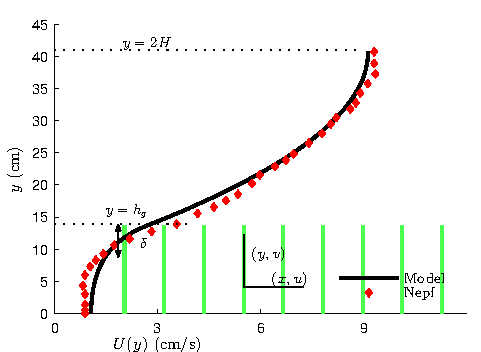
\includegraphics[scale=.99]{Grass_Base_Nepf} }
% 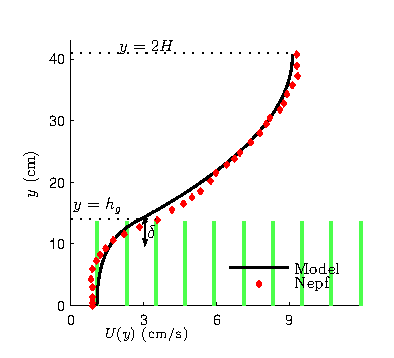
\includegraphics[width=15cm]{Grass_Base_Nepf_shear}
\caption{
Schematic setup and comparison of our steady flow profile with that from the experiments in ref. \cite{Nepf04} (Case I from Table 1) %  with 1250 plants/m$^2$, plant height = 13.7$\pm 0.2$ cm and blade width of 0.64 cm)
 and its approximation with $U_0=7.28$ cm/s and $\delta = 5.02$ cm in our model. The grass extends up to $y=\hg$ in the water column of depth $2H$. 
The steady velocity profile can be decomposed into a parabolic profile in the unvegetated region, a uniform profile deep within the vegetation, and a boundary layer of thickness $\delta$ near the grass top. 
The dependence of the boundary layer thickness (estimated as $|U/U_y|$ at $y=\hg$ from the numerical solution of \eqref{base_equ}) on the vegetation density parameter $\ReyNdg$ is shown in the inset.
}
\label{basicflow}
\end{figure}

Eq. \eqref{base_equ} is solved subject to no shear at the boundaries, i.e., $U'(0) = U'(2H) = 0$.
The former arises for dense vegetation because the shear stress exerted by the bottom surface is expected to be negligible compared to the vegetation drag (Nepf 2000 ) whereas the latter models the free interface. 
A comparison of the steady flow profile from the solution of ~\eqref{base_equ} with experimental measurements is shown in Fig.
The profile $U(y)$ has three distinct regions.
Within the vegetation, it is approximately uniform with $ U(y) \approx U_g = \sqrt{\frac{-dP/dx}{\rho C_N dN_g}}$, arising from a balance of the drag with the pressure gradient. 
Outside the vegetation, the velocity has a simple parabolic profile. % due to the balance between viscous forces and the pressure gradient. 
At the grass top, continuity of shear stresses results in a boundary layer of thickness $\delta$. 
Denoting $\ubl$ to be the velocity scale in the boundary layer, and $U_0 = {(-dP/dx)~H^2}/{\mu}$ the velocity scale in the unvegetated region, the balance between viscous forces and vegetation drag implies $(\mu \ubl/\delta^2 \sim \rho C_N d N_g \ubl^2)$, and the continuity of shear stress across the grass top implies $(\ubl/\delta \sim U_0/H)$.
Solving for $\delta$ and $\ubl$ yields $\delta/H \sim \ubl/U_0 \sim (\Rey \Ndg )^{-1/3}$, %where $\Ndg = \left(C_N d H N_g\right)$ is the vegetation frontal area per bed area, and $\Rey=\rho U_0 H/\mu$ is the Reynolds number of the flow. 
A numerical estimate of $\delta$ (estimated as $U/U_y$ at $y=\hg$) is compared with this prediction in Fig. \ref{basicflow} (inset).
We identify the boundary layer to be analogous to the shear layer {Ghisal02,Nepf04} in the previous explanation of \monami.
This dependence of $\delta$ on $N_g$ gives us a way to systematically investigate the effect of the shear layer thickness on the instability mechanism.
Fig. \ref{basicflow} also shows that the asymptotic regime of a thin boundary layer is expected to hold for $\ReyNdg \gtrsim 100$. 
In this notation, $U_g/U_0 = (\Rey \Ndg)^{-1/2}$ (used later in deriving \eqref{eqn:mode2asymp}). 
\begin{figure}
\centerline{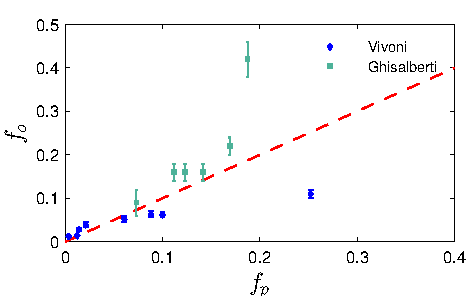
\includegraphics[]{new_graph_freq}}
\caption{Comparison of experimental observations of the experimentally measured dominant frequency $f_o$ (in Hz) with the predictions $f_p=\text{Im}(\sigma)$ from the solution of ~\eqref{Orr-somerfield}. 
The experimental data in the inset is obtained from \cite{Ghisal02} (Ghisalberti) and \cite{Vivoni98} (Vivoni). 
In order to estimate the $\Rey$ for these experiments, a representative value of $\mu=0.1$ Pa~s was assumed.
}
\label{frequency_comparison}
\end{figure}

Next we substitute $\bu = (U+\tilde{u}, \tilde{v})$, $p=P+\tilde{p}$ in ~\eqref{navier-stokes} and expand to linear order to investigate the evolution of small perturbations $(\tilde{u}, \tilde{v})$, which obey
\begin{equation}
\begin{split}
\rho(u_t+U u_x+vU_y) &= -p_x+ {\mu}\nabla^2u-2S\rho C_{N}dN_{g}Uu, \\
\rho(v_t+ Uv_x) &= -p_y+ {\mu}\nabla^2v, \hspace{0.3cm} \nabla\cdot\bu=0,
\end{split} \nonumber
\end{equation}
where the tilde are dropped.
These equations are non-dimensionalized using half channel height $H$, velocity $U_0$, and time $H/U_0$, leading to three non-dimensional parameters, \textit{viz.} $\Rey$, $\Ndg$, and the vegetation submergence ratio $\hg/H$. 
We also use $\delta/H$ in lieu of $\Ndg$ to parametrize the vegetation density and help elucidate the instability mechanism. 
Using a stream function $\psi$ with $u = \psi_{y}, v= -\psi_x$ to satisfy mass balance, we seek a solution of 
the form $\left(u,v,\psi \right)= \left(\hat u(y), \hat v(y), \phi(y) \right)e^{ikx+\sigma t}$ to obtain a modified Orr-Sommerfeld equation %\citep{Drazin81,Chen97,Chu91} 
\begin{figure}
 \centerline{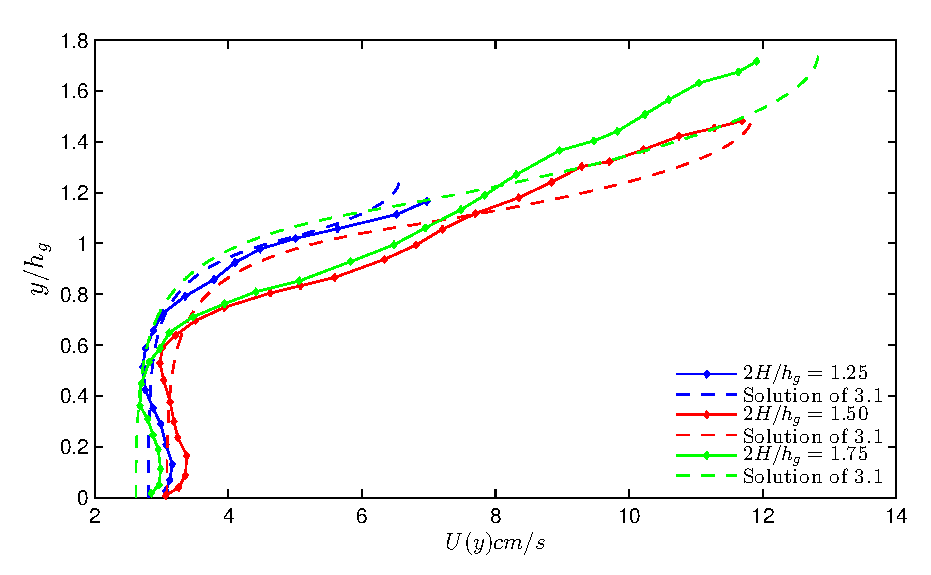
\includegraphics[]{Vivoni_Fig3_6_zero_shear_match} 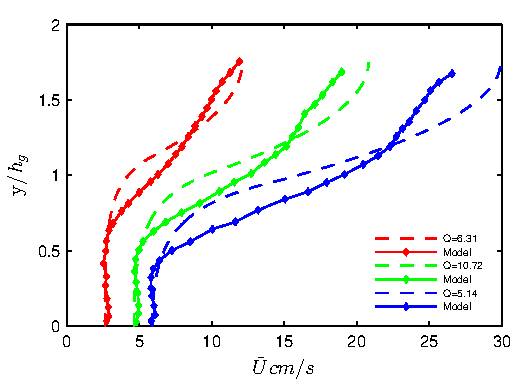
\includegraphics{Vivoni_Fig3_7_zero_shear_match}}
\end{figure}



\begin{equation}
\begin{split}
\Rey^{-1}\left(D^2 -k^{2} \right)^2\phi &= \left[ \left({\sigma}+ikU\right) \left(D^2-k^2\right) -ikU_{yy}\right]\phi + \Ndg D\left(2 S U D \phi\right),
\label{Orr-somerfield}
\end{split}
\end{equation}
where $D=d/dy$, and subject to the boundary conditions $\phi = D^2\phi = 0$ at $y=0$ and $y=2$. 
The growth rate $\sigma$ for a given wave number $k$ appears as an eigenvalue that allows a non-trivial solution $\phi$ of  \eqref{Orr-somerfield}.
We solve \eqref{Orr-somerfield} numerically for $\sigma$ and $\phi$.

%\lipsum[81-100]

\begin{figure}
  \centering
  \begin{tikzpicture}[scale=3]

  \draw [fill=red!20!white] (1,1) -- ++(0,-2) -- ++(-2,0) -- ++(0,2) -- cycle;
  \draw [fill=blue!20!white,opacity=0.4] (0,0) circle(2cm);
  \node [font={\Large\sf}] (yo) at (0,0) {Yo, yo, home slice};
  \draw[->,very thick, dashed] (yo) to [out=45,in=-45] (3,0);

\end{tikzpicture}

  \caption[Awesome picture]{Isn't this picture awesome?}
\end{figure}

\begin{figure}
  \centering
  \begin{tikzpicture}
  \draw [fill=red!70!white,circular drop shadow={shadow scale=1.05},very
  thick,rotate=45,opacity=0.7] (0,0) rectangle (3,2);


  \draw [fill=blue!70!white,circular drop shadow={shadow scale=1.05},very
  thick,rotate=135,opacity=0.7] (0,0) rectangle (3,2);
  \draw [fill=orange!70!white,circular drop shadow={shadow scale=1.05},very
  thick,rotate=225,opacity=0.7] (0,0) rectangle (3,2);
  \draw [fill=green!70!white,circular drop shadow={shadow scale=1.05},very
  thick,rotate=-45,opacity=0.7] (0,0) rectangle (3,2);
\end{tikzpicture}

  \caption[Tubular picture]{Totally tubular, dude}
\end{figure}

\clearpage{\pagestyle{empty}\cleardoublepage}

\chapter{The Main Event}
%\lipsum[101-120]

\clearpage{\pagestyle{empty}\cleardoublepage}

\chapter{Applying The Main Event}
%\lipsum[121-140]

\clearpage{\pagestyle{empty}\cleardoublepage}

\chapter{Conclusion}
%\lipsum[1-20]

\clearpage{\pagestyle{empty}\cleardoublepage}

%------------------------ APPENDIX ------------------------%
\appendix
\chapter{Stuff Too Complicated To Talk About}
%\lipsum[51-70]

\clearpage{\pagestyle{empty}\cleardoublepage}

\chapter{Stuff Too Boring to Talk About}
%\lipsum[111-130]

\clearpage{\pagestyle{empty}\cleardoublepage}

%---------------------- BIBLIOGRAPHY ----------------------%

\bibliographystyle{plain}
\begin{spacing}{0.9}
  \bibliography{thesis}
\end{spacing}

\end{document}
